\section{Mulighetsanalyse}

\subsection{Markedspotensial}

Primærkunden, den som eier problemet og har budsjettansvar, er Bane NOR SF. Brukerne er bane- og bruingeniører samt vedlikeholdspersonell som konsumerer tilstandsdata som grunnlag for prioritering og utbedring. I dag dekkes behovet gjennom årlige driftskontroller og ingeniørkontroller hvert sjette år, supplert med operatørstyrte droner og målevognen Roger~1000 (\cref{kontakt:traetten}). Ekstern inspeksjonskapasitet kjøpes fra aktører som Axess Group og droneoperatører på rammeavtale, men løsningene er arbeidsintensive og gir ikke et kontinuerlig tilstandsbilde (\cref{kontakt:eide}).

Konseptet skaper verdi langs tre akser. Kontinuerlig tilstandsovervåking muliggjør tidligere feildeteksjon og reduserer nedetid ved at begynnende skader fanges opp før de utvikler seg til driftsstans. Løsningen reduserer HMS-kostnader ved å fjerne personell fra spor og høye konstruksjoner, og adresserer samtidig sportilgangsutfordringen der inspeksjoner i dag presses til nattarbeid i togfrie perioder (\cref{kontakt:traetten}). Kontinuerlig dataanalyse gir i tillegg grunnlag for en overgang fra reaktivt til prediktivt vedlikehold.

Markedet segmenteres naturlig etter infrastrukturtype (bro, tunnel, fjellskjæring) og kritikalitet. Vi fokuserer på \emph{punktovervåking av høyrisikolokasjoner} fremfor flåtedekning, ettersom dagens dronebokser har begrenset rekkevidde og er lite egnet til lineær inspeksjon over lange strekninger (\cref{kontakt:wike}). Primærsegmentet er skred- og rasutsatte punkter, som Trætten fremhever som det mest prekære overvåkingsbehovet i Bane NOR og hvor det allerede er bevilget midler til en autonom dronestasjon på Meråkerbanen (\cref{kontakt:traetten}). Sekundært adresseres de mest kritiske av Bane NORs 2\,700+ broer~\cite{jernbanedirektoratet_tall}, særlig eldre stålbruer, overgangssoner og flomutsatte fundamenter (\cref{kontakt:sjetnan}), der eksakt omfang må kartlegges mot Bane NORs egen klassifisering i konsekvensklasser. Det globale markedet for dronebasert jernbaneinspeksjon er estimert til å vokse fra 1,67~mrd.~USD i 2025 til 4,86~mrd.~USD i 2030, tilsvarende en årlig vekst (CAGR) på om lag 24~\%~\cite{businessresearch_drone_2025}. Veksten drives av lettelser i BVLOS-regelverket, aldrende infrastruktur og modning av AI-drevne plattformer for prediktivt vedlikehold.

Når det gjelder prising, foreslår vi en hybrid modell: salg av dokkingstasjon og drone som engangskostnad på 1--1,5~MNOK per objekt, basert på referansetall fra Nordic Unmanned (\cref{kontakt:wike}), pluss et årlig abonnement på analyseplattform og drift anslått til 200--300~kNOK per objekt. Modellen reflekterer to sammenfallende preferanser: Bane NOR ønsker eierskap til utstyr og data (\cref{kontakt:traetten}), mens droneoperatørene foretrekker forutsigbare inntekter (\cref{kontakt:wike}). Betalingsvilje er empirisk bekreftet gjennom bevilgningen til Meråkerbanen-prosjektet. Samtidig illustrerer Nordic Unmanneds fireårige rammeavtale fra 2021, der forventet omsetning på 30~MNOK endte på om lag 436\,000~kr før selskapet gikk konkurs i februar 2025~\cite{aga_forventet_2025, dahl_droneselskap_2025}, at nominelle rammeavtaler med Bane NOR ikke automatisk konverterer til reell omsetning. Realistisk prising må derfor ta høyde for lav faktisk utnyttelse og lang ledetid fra signert avtale til fakturert aktivitet.


\subsection{Forretningsmodell, kommersialisering og økonomiske betraktninger}

\subsubsection{Forretningsmodellen}
\label{sec:forretningsmodell}

Kundesegmentet består primært av jernbaneinfrastrukturforvaltere med BaneNOR som første målgruppe. Verdien skapes gjennom økt inspeksjonsfrekvens, bedre beslutningsgrunnlag og redusert nedetid. Inntektsmodellen kan enten være en tjenestemodell (drone-as-a-service) eller en hybrid modell hvor kunden eier systemet og betaler for drift og analyse. Sistnevnte støttes av bransjeinnsikt som viser at kunder ofte ønsker eierskap til data og utstyr. Nøkkelressurser inkluderer dronebaser, AI-basert analyse og regulatorisk kompetanse, mens nøkkelpartnere vil være droneselskaper, teknologileverandører og juridiske aktører innen luftfartsregelverk.

\begin{figure}[ht]
    \centering
    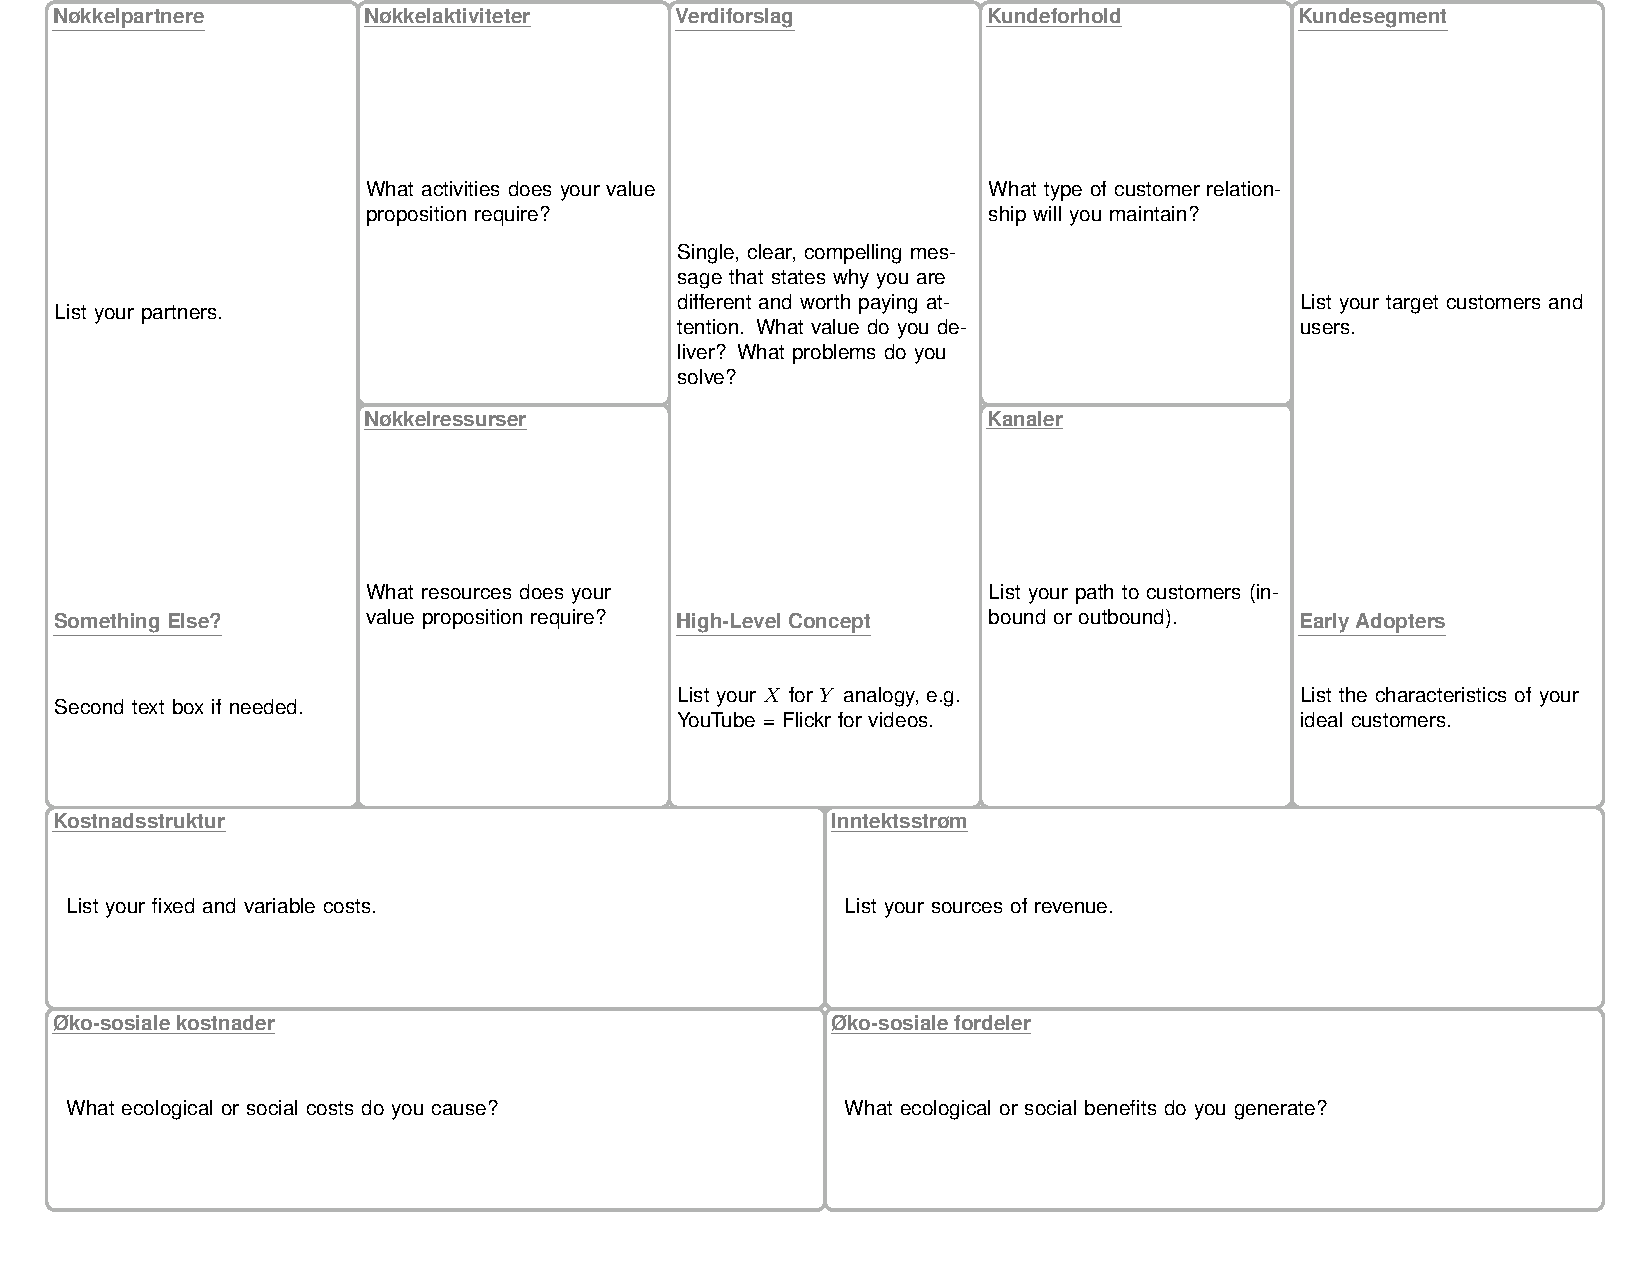
\includegraphics[width=1.0\linewidth]{figurer/Lerret_for_forretningsmodell.pdf}
    \caption{Utvidet \textit{Business Model Canvas} (lerret for forretningsmodell).}
    \label{fig:lerret-for-forretningsmodell}
\end{figure}

\subsubsection{Kommersialisering}
Kommersialiseringen vil skje stegvis, med pilotprosjekter ved utvalgte kritiske infrastrukturobjekter for å dokumentere effekt og redusere risiko. Dette er i tråd med eksisterende initiativer i bransjen hvor implementering av ny teknologi skjer gradvis og krever dokumentert nytteverdi. Videre skalering vil skje gjennom langsiktige kontrakter med infrastrukturforvaltere. Eventuelt i samarbeid med etablerte droneoperatører. Viktige barrierer inkluderer regulatoriske krav, særlig knyttet til BVLOS-operasjoner samt komplekse offentlige anskaffelsesprosesser. Konseptet befinner seg i en tidlig fase med høyt kapitalbehov og usikkerhet, men også et betydelig markedspotensial drevet av økende behov for effektiv og sikker infrastrukturforvaltning.

\subsubsection{Økonomiske betraktninger: kostnader, inntekter og finansiering}
\label{sec:okonomi}

Vår virksomhet kan klassifiseres som en vekstbedrift i idé- og utviklingsfasen, kjennetegnet av intensiv FoU, høy usikkerhet, betydelig kapitalbehov og omfattende ulønnet egeninnsats fra grunderne \parencite{torvatn_teknologiledelse_2024}. Det
økonomiske oppsettet består derfor av et drifts-, investerings- og likviditetsbudsjett for 2027, strukturert etter Altinns veileder for oppstartsbedrifter \parencite{altinn_budsjett} og retningslinjene i INGG2301. De fullstendige budsjettene er presentert i \cref{app:driftsbudsjett}.

Fem grundere tar delvis lønn på ca.\ 15\,000~NOK brutto per måned (20\,000~NOK inkl.\ sosiale kostnader per person, totalt 100\,000~NOK/mnd), mens resterende arbeidsinnsats er ulønnet egeninnsats. Investeringene på ca.\ 1,48~MNOK omfatter én prototypedrone (DJI~Matrice~350~RTK med Zenmuse~P1-payload), AI-utviklingsarbeidsstasjoner, testrigg og programvarelisenser, avskrevet lineært over fem år. Dokkingstasjoner og pilotinstallasjon utsettes til etablerings- og kommersialiseringsfasen i år 2--3. Samlede driftskostnader beløper seg til ca.\ 1,8~MNOK.

Utviklingsåret budsjetteres tilnærmet inntektsløst, slik læreboken beskriver som typisk for første driftsår i FoU-tunge virksomheter \parencite{torvatn_teknologiledelse_2024}. Vi budsjetterer kun 75\,000~NOK fra sporadiske konsulent- og rådgivningsoppdrag. Den hybride salgs- og abonnementsmodellen beskrevet i \cref{sec:forretningsmodell} aktiveres først ved pilotavtale i år~2.

Kapitalbehovet på ca.\ 3,3~MNOK dekkes av egenkapital, soft funding og kassakreditt. Tilskuddsbasert finansiering ble valgt fremfor aksjeemisjon for å bevare grundernes eierandeler og som ekstern kvalitetsvurdering av teknologien. Break-even-analysen indikerer at 2--3 dokkingstasjoner i stabil drift er tilstrekkelig for lønnsomhet.

Timingen er like kritisk som summen. SkatteFUNN-refusjonen på 500\,000~NOK inngår i finansieringsplanen, men utbetales først via skatteoppgjøret i år~2 og bidrar med null kroner til kontantstrømmen i 2027. Dette skaper et strukturelt underskudd gjennom hele året som forsterkes av CAPEX-tyngdepunktet i januar–mars. Likviditetsbudsjettet viser et maksimalt kassakredittbehov på ca.\ 1,57~MNOK i desember, som overstiger rammen på 1,3~MNOK med om lag 270\,000~NOK. Gapet kan lukkes gjennom leasing av drone, utsatt anskaffelse eller en fremskyndet utbetalingsprofil med Innovasjon Norge.